\documentclass[aspectratio=169, 12pt]{beamer}
\usepackage{bbm}
\usepackage[utf8]{inputenc}
\usepackage[T2A]{fontenc}
\usepackage[russian, english]{babel}
\usepackage{amscd,amssymb}
\usepackage{amsfonts,amsmath,array}
\usepackage{sidecap}
\usepackage[T2A]{fontenc}
\usepackage[utf8]{inputenc}
\usepackage{graphicx}				% Вставка картинок правильная
\graphicspath{{pictures/}, {images/}, {}}
\DeclareGraphicsExtensions{.pdf,.png,.jpg}
\usepackage{pdfpages}
\usepackage{multicol}

% Для алгоритмов
\usepackage{amsmath}
\usepackage{amsthm}
\usepackage{amssymb}
\usepackage{mathtools}
\usepackage{algorithm}
\usepackage{algpseudocode}
% Цвета 
\usepackage{color}
\usepackage{colortbl}

% Создаем новую команду для assumptions
%----------------------------------------------------------------------------------------------------------

\newtheorem{assumption}{Предположение}

%beamer  theme's used to be here :)
%\usetheme{mipt_beamer}
\usetheme{boxes}

%----------------------------------------------------------------------------------------------------------
\title[\hbox to 56mm{Feature}]{Методы с предобуславливанием и затуханием весов}
\author[М.\,В.~Крейнин]{Матвей Вадимович Крейнин}
\institute{Московский Физико-Технический Институт}

\date{
\footnotesize
\par\smallskip\emph{Кафедра:} Интеллектуальный анализ данных
\par\smallskip\emph{Научный руководитель:} кандидат ф.-м. наук А.\,Н.~Безносиков
\par\bigskip\small 2024}

\begin{document}
\maketitle

\begin{frame}{Постановка задачи}

    Минимизация функции:
    \begin{equation}
    \label{eq:general}
        \min_{w \in \mathbb{R}^d} f(w)
    \end{equation} 
    Классическое решение проблемы минимизации функции в машинном обучении:
    \begin{equation*}
        w_t = w_{t-1} - \eta \nabla f(w_t).
    \end{equation*}

    Алгоритмы с предобуславливанием:
    \begin{equation*}
        w_{t+1} = w_t - \eta D_t^{-1}g_t
    \end{equation*}
    где $g_t$ это несмещённый стохастический градиент, $D_t$ это матрица предобуславливания.
\end{frame}

\begin{frame}{Различные способы задания матрицы }
    AdaGrad:
    \begin{equation*}
        D_t = diag \left\{\sqrt{\sum\limits_{i=0}^t g_i \odot g_i} \right\}
    \end{equation*}
    RMSProp and Adam:
    \begin{equation*}
        D_t^2 = \beta D_{t-1}^2 + (1-\beta) diag \{g_t \odot g_t \}
    \end{equation*}
    OASIS:
    \begin{equation*}
        D_t = diag \{z \odot \nabla^2 f(w_t) z\}
    \end{equation*}
    где $z$ это случайный вектор из распределения Рандемахера.
\end{frame}


\begin{frame}[shrink]{Новая минимизируемая функция}
\begin{equation*}
        \min_{w \in \mathbb{R}^d} F(w) := f(w) + r(w)
\end{equation*}
где $r(w)$ это функция регуляризации.

\begin{algorithm}[H]
    \caption{Различные способы использования предобуславливания с регуляризацией}
    \label{alg:precond}
    
    \begin{algorithmic}
            \Require{$\eta$ $-$ шаг обучения, $f$ $-$ оптимзируемая функция}
            
            \While {$w$ не сойдется}
            \State $t = t+1$
            \State $g_t \gets$ стохастический градиент $f$
            \State $\textcolor{blue}{g_t \gets g_t + \nabla r(w_t)}$ \hfill \textcolor{blue}{обычная регуляризация}
            \State $D_t \gets$ матрица предобуславливания с помощью $g_t$

            \State \textcolor{blue}{$w_t \gets w_{t-1} - \eta \cdot D_t^{-1}g_t $} \hfill \textcolor{blue}{обычная регуляризация}, 
            \State \textcolor{orange}{$w_t \gets w_{t-1} - \eta \cdot D_t^{-1} \left(g_t +\nabla r(w_t) \right)$} \hfill \textcolor{orange}{масштабированное затухание весов}, 
            \State \textcolor{red}{$w_t \gets w_{t-1} - \eta \cdot D_t^{-1} g_t  - \eta \cdot \nabla r(w_t)$} \hfill \textcolor{red}{затухание весов}, 
            \EndWhile
    \end{algorithmic}
\end{algorithm}

\end{frame}

\begin{frame}{Альтернативный взгляд}

Вынесем $D_t^{-1}$ за скобки и получим новый градиент:
\begin{equation*}
    w_{t+1} = w_t - \eta D_t^{-1}(\nabla f(w_t) + D_t \nabla r(w_t))
\end{equation*}
Новая функция регуляризации $\nabla \tilde{r}(w) = D_t \nabla r(w)$.


Задача минимизации, которая решается на самом деле:
\begin{equation*}
\label{F_tilde}
    \min_{w \in \mathbb{R}^d} \tilde{F}(w) := f(w) + \tilde{r}(w)
\end{equation*}
где $\tilde{F}(w)$ изменяется на каждом шаге.
\end{frame}

\begin{frame}{Предположения на функции}

\begin{assumption}{(Структура регулязитора)}
    \label{ass:regstruct}
    Регуляризатор $r$ сепарабелен, то есть он может быть представлен в следующем виде:
    $r(w) = \sum_{i=1}^d r_i(w^i),$
    где $r_i(x) \ge 0$ для $i \in \overline{1, d}$ и $x \in \mathbb{R}$.
\end{assumption}

\begin{assumption}{(Структура матрицы предобуславливания)}
    \label{ass:precondstruct}
    Матрица предобуславливания $D_t$ может быть представлена в следующем виде:
     $D_t = \textrm{diag} \left\{ d_t^1 \ldots, d
_t^d \right\}.$
\end{assumption}
\begin{assumption}{(Сильная выпуклость)}
    \label{ass:muconvex}
    Сушествует $\mu_f$ такая, что $\forall x, y \in \mathbb{R}^d$ выполняется:
    $$
    f(y) \geq f(x) + \langle \nabla f(x), y-x \rangle + \frac{\mu_f}{2} ||x-y||_2^2
    $$
\end{assumption}
\end{frame}

\begin{frame}{Предположения на функции}
    \begin{assumption}{($L$-гладкость)} 
\label{ass:smoothness}
\begin{itemize}
    \item 	Градиент функции $f$ является $L_f$-гладким, то есть существует такая константа $L_f > 0$ такая, что $\forall x, y \in \mathbb{R}^d$,
    	\begin{equation*}
    		f(x) \leq f(y) + \langle \nabla f(y), x-y \rangle + \frac{L_f}{2} \|x - y\|^2.
    	\end{equation*}
    \item    Градиент функции $r$ является $L_r$-гладким, то есть существует такая константа $L_r > 0$ такая, что $\forall x, y \in \mathbb{R}^d$,
	\begin{equation*}
		r(x) \leq r(y) + \langle \nabla r(y), x-y \rangle + \frac{L_r}{2} ||x - y||^2.
	\end{equation*}
\end{itemize}
\end{assumption}

\end{frame}

\begin{frame}[shrink]{Предположения на функции}
\begin{assumption}{(Ограниченность регуляризатора)}
\label{ass:regbound}
Регуляризатор ограничен, то есть существует константа $\Omega > 0$ такая, что $\forall w \in \mathbb{R}^d$ выполняется $ |r(w)| \le \Omega.$
\end{assumption}

\begin{assumption}{(Ограниченность предобуславливателя)}
\label{ass:preconditioned}
Существуют константы $\alpha, \Gamma \in \mathbb{R} : 0 < \alpha < \Gamma$ такие, что
\begin{equation*}
\alpha I \preccurlyeq D_t \preccurlyeq \Gamma I \Leftrightarrow \frac{I}{\Gamma} \preccurlyeq D_t^{-1} \preccurlyeq \frac{I}{\alpha}.
\end{equation*}
\end{assumption}

\begin{assumption}{(Ожидания)}
\label{ass:expectations}
$g_t$ являются несмещенными и имеют ограниченную вариацию на любом шаге, то есть
\begin{equation*}
\mathbb{E}\left[ g_t \right] = \nabla f (w_t), \mathbb{E}\left[ ||g_t - \nabla f||^2 \right] \leq \sigma^2.
\end{equation*}
\end{assumption}

\end{frame}

\begin{frame}{Леммы}
    \begin{lemma}
\label{lemma:existence}
{(Существование $\widetilde{r}$)}
    Предполагая, что \ref{ass:regstruct}, \ref{ass:precondstruct} выполняются, функция $\widetilde{r}$ существует и имеет следующую форму:
    $$\widetilde{r}_t(w) = \sum_{i=1}^d d_t^i r_i(w_i)$$
\end{lemma}

\begin{lemma}\label{lemma:tildesmoothness}{(L-гладкость $\widetilde{r}$)}
Предполагая, что \ref{ass:regstruct}, \ref{ass:precondstruct}, \ref{ass:smoothness}, \ref{ass:preconditioned} выполняются,
градиент $\widetilde{r}$ является $L_{\tilde{r}}$-непрерывным, 
то есть существует константа  $L_{\tilde{r}} > 0$ такая, что $\forall x, y \in \mathbb{R}^d$,
\begin{equation*}
    		\widetilde{r}_t(x) \leq \widetilde{r}_t(y) + \langle \nabla \widetilde{r}_t(y), x-y \rangle + \frac{L_{\tilde{r}}}{2} ||x - y||^2,
    	\end{equation*}
     и $L_{\tilde{r}} = \Gamma L_r$.
\end{lemma}


\end{frame}


\begin{frame}{Теоремы}
\begin{theorem} 
    \label{theor:1}
    Предполагая, что \ref{ass:regstruct}, \ref{ass:precondstruct}, \ref{ass:smoothness}, \ref{ass:regbound}, \ref{ass:preconditioned} выполняются, положим ошибку $\varepsilon > 0$ и шаг обучения удовлетворяют условию:
    $    \eta < \frac{2 \alpha}{L_f + \Gamma L_{r}}$,
    где $L_f, L_{r}$ - константа Липшица функций $f$ и $r$. 
    Необходимое количество итераций, начиная с начальной точки
    $w_0 \in \mathbb{R}^d$ с $\Delta_0 = \tilde{F}_0(w_0) - f^*$, где $\widetilde{F}_t$ определено в \eqref{F_tilde} и $f^*$ решением задачи \eqref{eq:general}, 
    необходимое для $\varepsilon$-приближения    
    \begin{equation*}
      T = \mathcal{O}\left( \frac{\Delta_0 \Gamma}{(\eta - \frac{\tilde{L}\eta^2}{2\alpha}) \left( \varepsilon -\frac{\delta\Gamma}{\eta - \frac{\tilde{L}\eta^2}{2\alpha}}\right)} \right),
\end{equation*}
где $\widetilde{L} = L_f + \Gamma L_{r}$ and $\delta$ может выбрано сколь угодно малым с помощью выбора гиперпараметров $\alpha, \beta, \Gamma$
\end{theorem}
\end{frame}

\begin{frame}{Теоремы}
    \begin{theorem}
\label{theor:2}
    Преполагая, что \ref{ass:regstruct}, \ref{ass:precondstruct}, \ref{ass:smoothness}, \ref{ass:regbound}, \ref{ass:preconditioned}, \ref{ass:muconvex} выполняются, положим ошибку $\varepsilon > 0$ и шаг обучения удовлетворяют условию: $\eta < \frac{\alpha}{4L_f}$, гиперпараметры удовлетворяют условиям: $\lambda < \frac{\alpha \beta^2}{8L_f \Omega_0^2}$, $\beta \geq 1 - \frac{\eta(\mu_f + \lambda)\alpha}{2 \Gamma^2}$, $\Omega_0^2 \geq \frac{\alpha^2 \beta^2}{8L_f^2}$. Получаем оценку на необходимое количество шагов для сходимости алгоритма к заданной точности

   $$
T = \max \left\{ \log{\left( \frac{4 \varepsilon (1-\beta) L_f^2 }{\alpha \beta^2} \right)} \cdot \log{\frac{2}{1+\beta}} ;
\frac{4}{\frac{\alpha}{4L_f} \left(\mu_f + \frac{\alpha \beta^2}{8L_f \Omega_0^2} \right)}\log{\left(\frac{2 ||w_0-w_*||_2^2}{\varepsilon} \right)} \right\}
$$
\end{theorem}
\end{frame}

\begin{frame}{AdamW}
    \begin{algorithm}[H]
            \caption{Adam}\label{alg:genAdam}    
            \begin{algorithmic}
            \small{
            \Require{$\eta, \beta_1, \beta_2, \epsilon, f, r$}
            %\State $m_0 = 0$ -- 1-st moment vector
            %\State$v_0 = 0$ -- 2-nd moment vector
            \While {$\theta$ not converged}
            \State $t = t+1$
            \State $g_t = \nabla f(w_{t-1}) + $ \textcolor{blue}{$\nabla r(w_{t-1})$}\hfill \textcolor{blue}{AdamL2}
            \State $m_t = \beta_1 \cdot m_{t-1} + (1 - \beta_1) \cdot g_t$
            \State $v_t = \beta_2 \cdot v_{t-1} + (1 - \beta_2) \cdot g_t^2$
            \State $\hat{m_t} = \frac{m_t}{1-\beta_1^t} +$ \textcolor{orange}{$\nabla r(w_{t-1})$} \hfill \textcolor{orange}{AdamWH}
            \State $\hat{v_t} = \frac{v_t}{1-\beta_2^t}$ 
            \State $w_t = w_{t-1} - \eta \cdot \frac{\hat{m_t}}{\sqrt{v_t} + \epsilon} - $ \textcolor{red}{$\eta \nabla r(w_{t-1})$ } \hfill \textcolor{red}{AdamW}
            \EndWhile
            }
\end{algorithmic}
\end{algorithm}
\end{frame}

\begin{frame}{OASIS}
    \begin{algorithm}[H]
\caption{OASIS}\label{alg:OASIS}
\begin{algorithmic}
    \Require{$w_0, \eta_0, D_0, \theta_0 = + \infty$}    
    \State $w_1 = w_0 - \eta \hat{D_0}^{-1} \nabla f(w_0)$

    \For{$k = 1, 2, ...$}
    \State $g_k = \nabla f(w_k) +$ \textcolor{blue}{$\nabla r(w_{t-1})$}\hfill \textcolor{blue}{OASISL2} 
    \State $D_k = \beta D_{k-1} + (1-\beta_2) \cdot diag\left( z_k \odot \nabla^2 \left(f(w_k) + \textcolor{orange}{r(w_k)} \right) z_k \right)$ \hfill \textcolor{orange}{OASISWH}
    \State $(\hat{D_k})_{ii} = max \{|D_k|_{i, i} ; \alpha \}$, $\forall i = \overline{1, d}$
    \State $\eta_k = min \{ \sqrt{1 + \theta_{k-1}} \cdot \eta_{k-1}; \frac{||w_k - w_{k-1}||_{\hat{D_k}}}{2 ||\nabla f(w_k) - \nabla f(w_{k-1}) ||_{\hat{D_k}}^* } \}$
    \State $w_{k+1} = w_k - \eta_k g_k D_k^{-1}- $ \textcolor{red}{$\eta \nabla r(w_{t-1})$ } \hfill \textcolor{red}{OASISW} 
    \State $\theta_k = \frac{\eta_k}{\eta_{k-1}}$
    \EndFor
    
\end{algorithmic}
\end{algorithm}
\end{frame}

\begin{frame}{Experiments}
\begin{figure}[H]
\begin{minipage}[h]{0.49\linewidth}
\centering

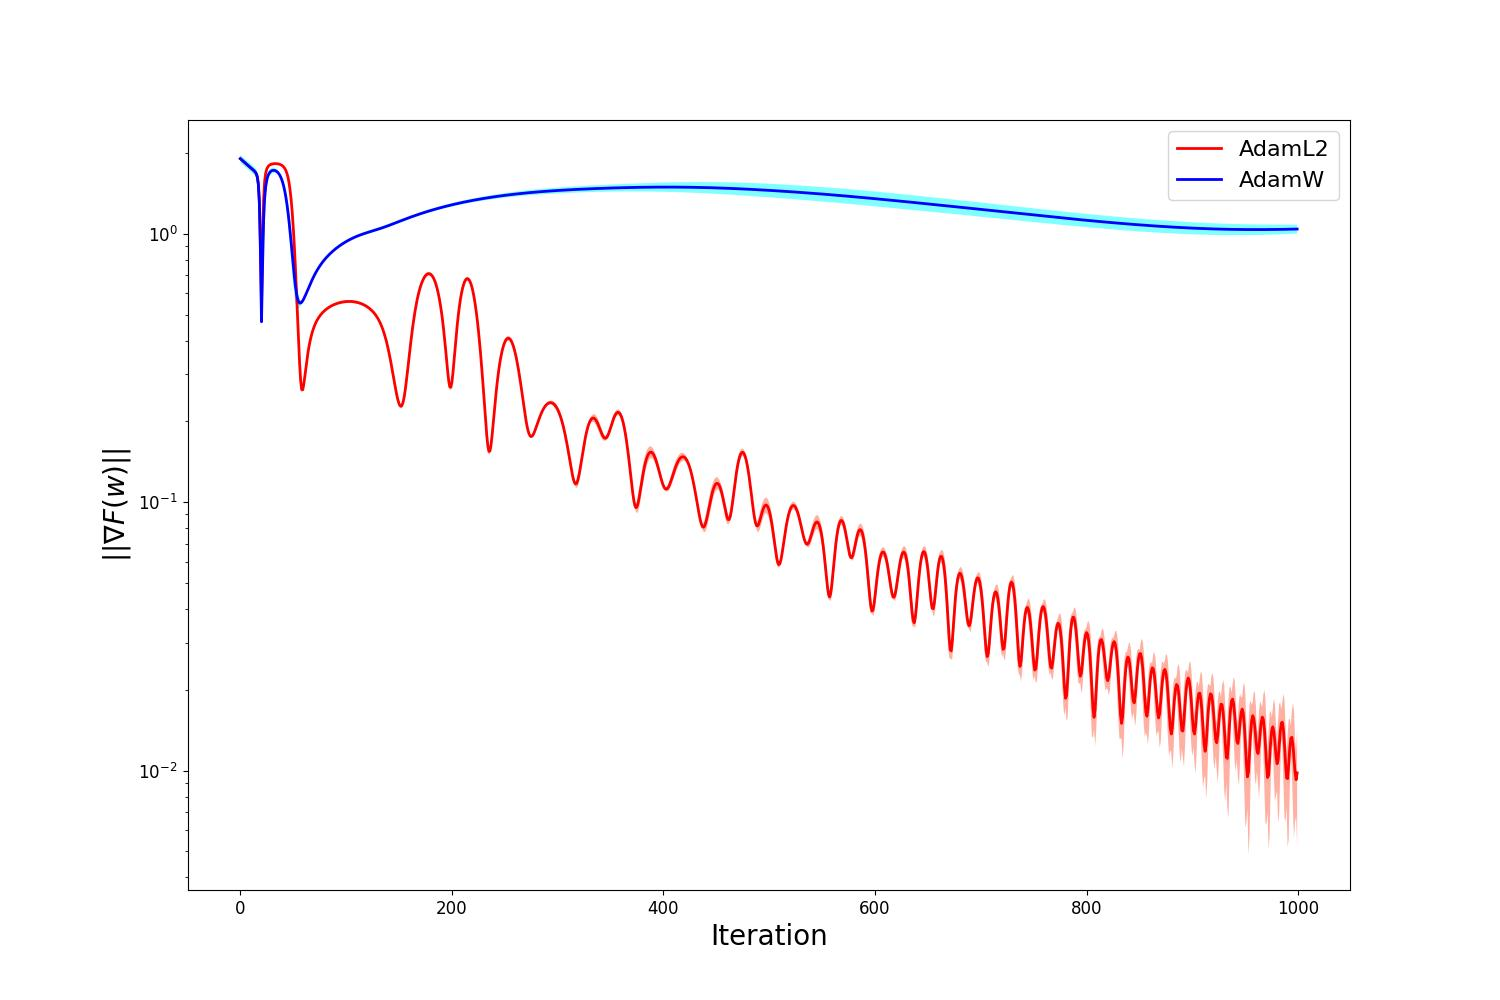
\includegraphics[width=\linewidth]{fig1.jpg}

\caption{Adam and AdamW with basic criterion}
\label{fig:adams_errors}
\end{minipage}
\hfill
\begin{minipage}[h]{0.49\linewidth}
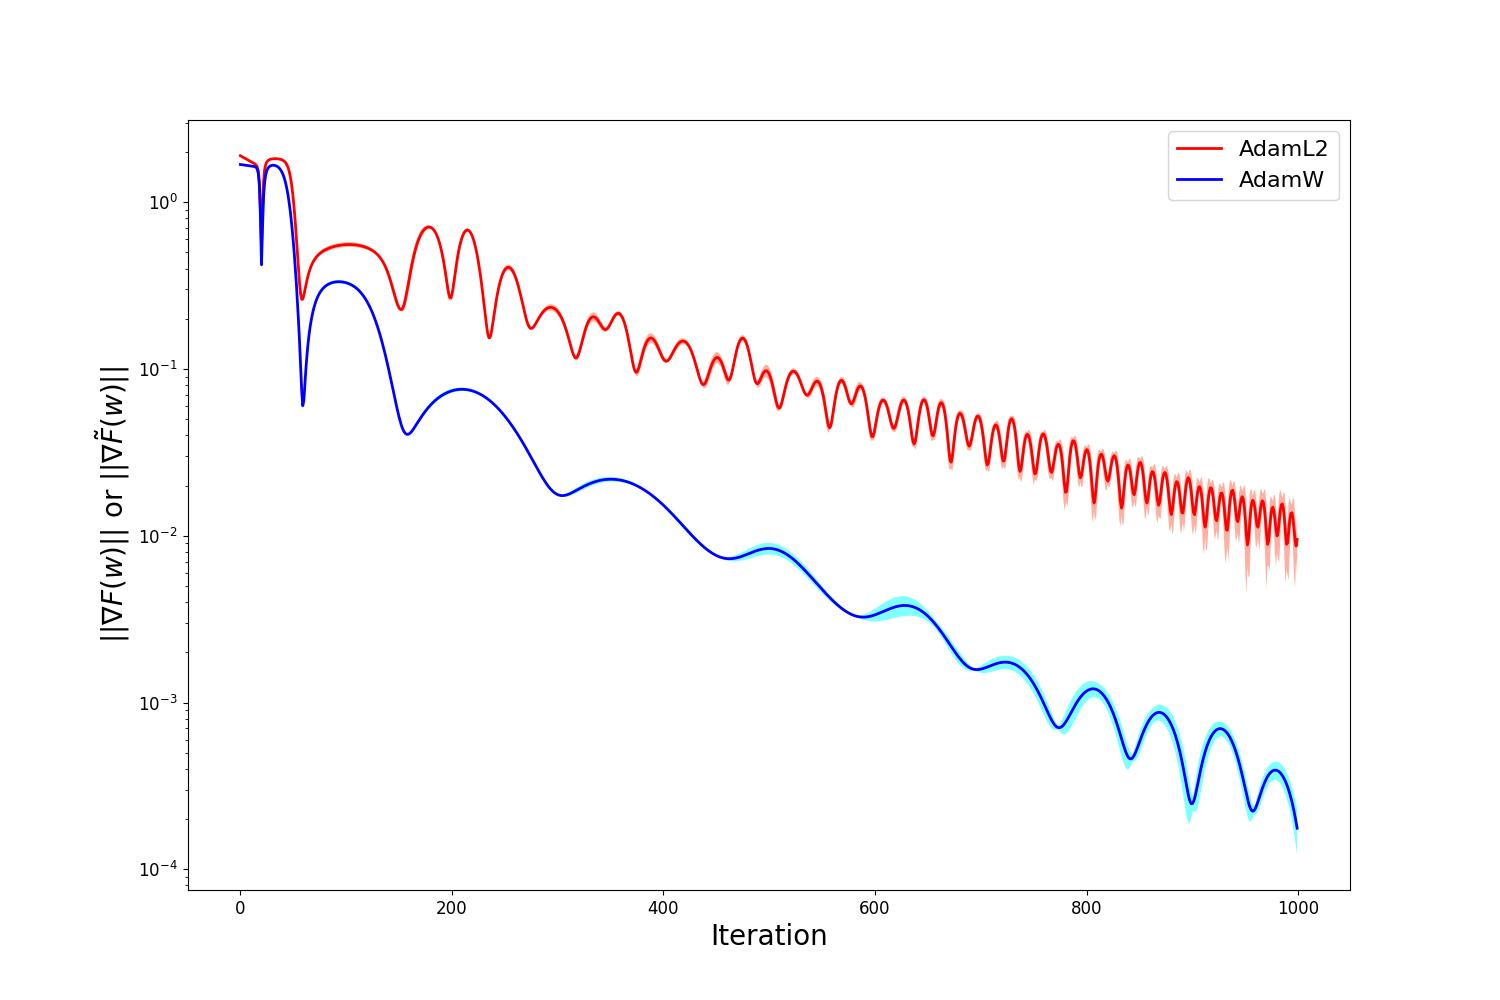
\includegraphics[width=\linewidth]{fig2.jpg}
\caption{Adam and AdamW with modified criterion}
\label{fig:adams_special_errors}
\end{minipage}
\end{figure}
\end{frame}



\begin{frame}{Список литературы}
    \begin{itemize}
        \item Kingma, Diederik P., and Jimmy Ba. "Adam: A method for stochastic optimization." arXiv preprint arXiv:1412.6980 (2014).
        \item Jahani, Majid, et al. "Doubly adaptive scaled algorithm for machine learning using second-order information." arXiv preprint arXiv:2109.05198 (2021).
        \item Sadiev, Abdurakhmon, et al. "Stochastic gradient methods with preconditioned updates." arXiv preprint arXiv:2206.00285 (2022).
        \item Beznosikov, Aleksandr, et al. "On scaled methods for saddle point problems." arXiv preprint arXiv:2206.08303 (2022).
        \item Loshchilov, Ilya, and Frank Hutter. "Decoupled weight decay regularization." arXiv preprint arXiv:1711.05101 (2017).
        \item Xie, Zeke, Issei Sato, and Masashi Sugiyama. "Stable weight decay regularization." (2020).
    \end{itemize}
\end{frame}

\begin{frame}{Заключение}
    \begin{itemize}
        \item Исследована теоретическая сходимость методов.
        \item Предложен новый метод добавления регуляризатора в методы с предобуславливанием.
        \item Доказаны две теоремы и две леммы.
    \end{itemize}
\end{frame}


\end{document}